\documentclass[1p]{elsarticle_modified}
%\bibliographystyle{elsarticle-num}

%\usepackage[colorlinks]{hyperref}
%\usepackage{abbrmath_seonhwa} %\Abb, \Ascr, \Acal ,\Abf, \Afrak
\usepackage{amsfonts}
\usepackage{amssymb}
\usepackage{amsmath}
\usepackage{amsthm}
\usepackage{scalefnt}
\usepackage{amsbsy}
\usepackage{kotex}
\usepackage{caption}
\usepackage{subfig}
\usepackage{color}
\usepackage{graphicx}
\usepackage{xcolor} %% white, black, red, green, blue, cyan, magenta, yellow
\usepackage{float}
\usepackage{setspace}
\usepackage{hyperref}

\usepackage{tikz}
\usetikzlibrary{arrows}

\usepackage{multirow}
\usepackage{array} % fixed length table
\usepackage{hhline}

%%%%%%%%%%%%%%%%%%%%%
\makeatletter
\renewcommand*\env@matrix[1][\arraystretch]{%
	\edef\arraystretch{#1}%
	\hskip -\arraycolsep
	\let\@ifnextchar\new@ifnextchar
	\array{*\c@MaxMatrixCols c}}
\makeatother %https://tex.stackexchange.com/questions/14071/how-can-i-increase-the-line-spacing-in-a-matrix
%%%%%%%%%%%%%%%

\usepackage[normalem]{ulem}

\newcommand{\msout}[1]{\ifmmode\text{\sout{\ensuremath{#1}}}\else\sout{#1}\fi}
%SOURCE: \msout is \stkout macro in https://tex.stackexchange.com/questions/20609/strikeout-in-math-mode

\newcommand{\cancel}[1]{
	\ifmmode
	{\color{red}\msout{#1}}
	\else
	{\color{red}\sout{#1}}
	\fi
}

\newcommand{\add}[1]{
	{\color{blue}\uwave{#1}}
}

\newcommand{\replace}[2]{
	\ifmmode
	{\color{red}\msout{#1}}{\color{blue}\uwave{#2}}
	\else
	{\color{red}\sout{#1}}{\color{blue}\uwave{#2}}
	\fi
}

\newcommand{\Sol}{\mathcal{S}} %segment
\newcommand{\D}{D} %diagram
\newcommand{\A}{\mathcal{A}} %arc


%%%%%%%%%%%%%%%%%%%%%%%%%%%%%5 test

\def\sl{\operatorname{\textup{SL}}(2,\Cbb)}
\def\psl{\operatorname{\textup{PSL}}(2,\Cbb)}
\def\quan{\mkern 1mu \triangleright \mkern 1mu}

\theoremstyle{definition}
\newtheorem{thm}{Theorem}[section]
\newtheorem{prop}[thm]{Proposition}
\newtheorem{lem}[thm]{Lemma}
\newtheorem{ques}[thm]{Question}
\newtheorem{cor}[thm]{Corollary}
\newtheorem{defn}[thm]{Definition}
\newtheorem{exam}[thm]{Example}
\newtheorem{rmk}[thm]{Remark}
\newtheorem{alg}[thm]{Algorithm}

\newcommand{\I}{\sqrt{-1}}
\begin{document}

%\begin{frontmatter}
%
%\title{Boundary parabolic representations of knots up to 8 crossings}
%
%%% Group authors per affiliation:
%\author{Yunhi Cho} 
%\address{Department of Mathematics, University of Seoul, Seoul, Korea}
%\ead{yhcho@uos.ac.kr}
%
%
%\author{Seonhwa Kim} %\fnref{s_kim}}
%\address{Center for Geometry and Physics, Institute for Basic Science, Pohang, 37673, Korea}
%\ead{ryeona17@ibs.re.kr}
%
%\author{Hyuk Kim}
%\address{Department of Mathematical Sciences, Seoul National University, Seoul 08826, Korea}
%\ead{hyukkim@snu.ac.kr}
%
%\author{Seokbeom Yoon}
%\address{Department of Mathematical Sciences, Seoul National University, Seoul, 08826,  Korea}
%\ead{sbyoon15@snu.ac.kr}
%
%\begin{abstract}
%We find all boundary parabolic representation of knots up to 8 crossings.
%
%\end{abstract}
%\begin{keyword}
%    \MSC[2010] 57M25 
%\end{keyword}
%
%\end{frontmatter}

%\linenumbers
%\tableofcontents
%
\newcommand\colored[1]{\textcolor{white}{\rule[-0.35ex]{0.8em}{1.4ex}}\kern-0.8em\color{red} #1}%
%\newcommand\colored[1]{\textcolor{white}{ #1}\kern-2.17ex	\textcolor{white}{ #1}\kern-1.81ex	\textcolor{white}{ #1}\kern-2.15ex\color{red}#1	}

{\Large $\underline{12n_{0448}~(K12n_{0448})}$}

\setlength{\tabcolsep}{10pt}
\renewcommand{\arraystretch}{1.6}
\vspace{1cm}\begin{tabular}{m{100pt}>{\centering\arraybackslash}m{274pt}}
\multirow{5}{120pt}{
	\centering
	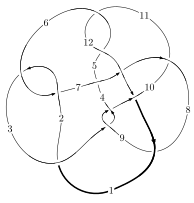
\includegraphics[width=112pt]{../../../GIT/diagram.site/Diagrams/png/2537_12n_0448.png}\\
\ \ \ A knot diagram\footnotemark}&
\allowdisplaybreaks
\textbf{Linearized knot diagam} \\
\cline{2-2}
 &
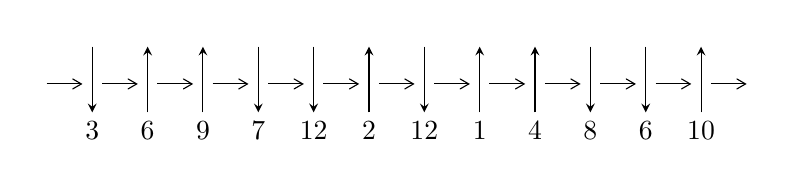
\begin{tikzpicture}[x=20pt, y=17pt]
	% nodes
	\node (C0) at (0, 0) {};
	\node (C1) at (1, 0) {};
	\node (C1U) at (1, +1) {};
	\node (C1D) at (1, -1) {3};

	\node (C2) at (2, 0) {};
	\node (C2U) at (2, +1) {};
	\node (C2D) at (2, -1) {6};

	\node (C3) at (3, 0) {};
	\node (C3U) at (3, +1) {};
	\node (C3D) at (3, -1) {9};

	\node (C4) at (4, 0) {};
	\node (C4U) at (4, +1) {};
	\node (C4D) at (4, -1) {7};

	\node (C5) at (5, 0) {};
	\node (C5U) at (5, +1) {};
	\node (C5D) at (5, -1) {12};

	\node (C6) at (6, 0) {};
	\node (C6U) at (6, +1) {};
	\node (C6D) at (6, -1) {2};

	\node (C7) at (7, 0) {};
	\node (C7U) at (7, +1) {};
	\node (C7D) at (7, -1) {12};

	\node (C8) at (8, 0) {};
	\node (C8U) at (8, +1) {};
	\node (C8D) at (8, -1) {1};

	\node (C9) at (9, 0) {};
	\node (C9U) at (9, +1) {};
	\node (C9D) at (9, -1) {4};

	\node (C10) at (10, 0) {};
	\node (C10U) at (10, +1) {};
	\node (C10D) at (10, -1) {8};

	\node (C11) at (11, 0) {};
	\node (C11U) at (11, +1) {};
	\node (C11D) at (11, -1) {6};

	\node (C12) at (12, 0) {};
	\node (C12U) at (12, +1) {};
	\node (C12D) at (12, -1) {10};
	\node (C13) at (13, 0) {};

	% arrows
	\draw[->,>={angle 60}]
	(C0) edge (C1) (C1) edge (C2) (C2) edge (C3) (C3) edge (C4) (C4) edge (C5) (C5) edge (C6) (C6) edge (C7) (C7) edge (C8) (C8) edge (C9) (C9) edge (C10) (C10) edge (C11) (C11) edge (C12) (C12) edge (C13) ;	\draw[->,>=stealth]
	(C1U) edge (C1D) (C2D) edge (C2U) (C3D) edge (C3U) (C4U) edge (C4D) (C5U) edge (C5D) (C6D) edge (C6U) (C7U) edge (C7D) (C8D) edge (C8U) (C9D) edge (C9U) (C10U) edge (C10D) (C11U) edge (C11D) (C12D) edge (C12U) ;
	\end{tikzpicture} \\
\hhline{~~} \\& 
\textbf{Solving Sequence} \\ \cline{2-2} 
 &
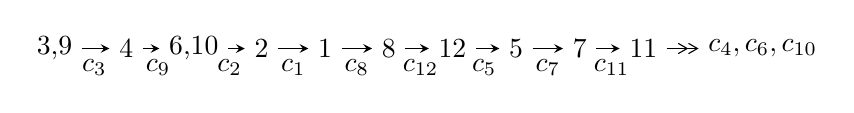
\begin{tikzpicture}[x=23pt, y=7pt]
	% node
	\node (A0) at (-1/8, 0) {3,9};
	\node (A1) at (1, 0) {4};
	\node (A2) at (33/16, 0) {6,10};
	\node (A3) at (25/8, 0) {2};
	\node (A4) at (33/8, 0) {1};
	\node (A5) at (41/8, 0) {8};
	\node (A6) at (49/8, 0) {12};
	\node (A7) at (57/8, 0) {5};
	\node (A8) at (65/8, 0) {7};
	\node (A9) at (73/8, 0) {11};
	\node (C1) at (1/2, -1) {$c_{3}$};
	\node (C2) at (3/2, -1) {$c_{9}$};
	\node (C3) at (21/8, -1) {$c_{2}$};
	\node (C4) at (29/8, -1) {$c_{1}$};
	\node (C5) at (37/8, -1) {$c_{8}$};
	\node (C6) at (45/8, -1) {$c_{12}$};
	\node (C7) at (53/8, -1) {$c_{5}$};
	\node (C8) at (61/8, -1) {$c_{7}$};
	\node (C9) at (69/8, -1) {$c_{11}$};
	\node (A10) at (11, 0) {$c_{4},c_{6},c_{10}$};

	% edge
	\draw[->,>=stealth]	
	(A0) edge (A1) (A1) edge (A2) (A2) edge (A3) (A3) edge (A4) (A4) edge (A5) (A5) edge (A6) (A6) edge (A7) (A7) edge (A8) (A8) edge (A9) ;
	\draw[->>,>={angle 60}]	
	(A9) edge (A10);
\end{tikzpicture} \\ 

\end{tabular} \\

\footnotetext{
The image of knot diagram is generated by the software ``\textbf{Draw programme}" developed by Andrew Bartholomew(\url{http://www.layer8.co.uk/maths/draw/index.htm\#Running-draw}), where we modified some parts for our purpose(\url{https://github.com/CATsTAILs/LinksPainter}).
}\phantom \\ \newline 
\centering \textbf{Ideals for irreducible components\footnotemark of $X_{\text{par}}$} 
 
\begin{align*}
I^u_{1}&=\langle 
-5.53148\times10^{174} u^{69}-2.38859\times10^{175} u^{68}+\cdots+3.44094\times10^{175} b-1.21041\times10^{177},\\
\phantom{I^u_{1}}&\phantom{= \langle  }2.30131\times10^{177} u^{69}+1.00000\times10^{178} u^{68}+\cdots+6.43455\times10^{177} a+4.92351\times10^{179},\\
\phantom{I^u_{1}}&\phantom{= \langle  }u^{70}+5 u^{69}+\cdots+133 u+187\rangle \\
I^u_{2}&=\langle 
-1290033 u^{15}-1131359 u^{14}+\cdots+1197778 b+2926203,\\
\phantom{I^u_{2}}&\phantom{= \langle  }953271 u^{15}+281899 u^{14}+\cdots+1197778 a-2560769,\\
\phantom{I^u_{2}}&\phantom{= \langle  }u^{16}-4 u^{14}+7 u^{13}+6 u^{12}-35 u^{11}+5 u^{10}+78 u^9-22 u^8-81 u^7+26 u^6+40 u^5-9 u^4-8 u^3- u^2+1\rangle \\
\\
\end{align*}
\raggedright * 2 irreducible components of $\dim_{\mathbb{C}}=0$, with total 86 representations.\\
\footnotetext{All coefficients of polynomials are rational numbers. But the coefficients are sometimes approximated in decimal forms when there is not enough margin.}
\newpage
\renewcommand{\arraystretch}{1}
\centering \section*{I. $I^u_{1}= \langle -5.53\times10^{174} u^{69}-2.39\times10^{175} u^{68}+\cdots+3.44\times10^{175} b-1.21\times10^{177},\;2.30\times10^{177} u^{69}+1.00\times10^{178} u^{68}+\cdots+6.43\times10^{177} a+4.92\times10^{179},\;u^{70}+5 u^{69}+\cdots+133 u+187 \rangle$}
\flushleft \textbf{(i) Arc colorings}\\
\begin{tabular}{m{7pt} m{180pt} m{7pt} m{180pt} }
\flushright $a_{3}=$&$\begin{pmatrix}1\\0\end{pmatrix}$ \\
\flushright $a_{9}=$&$\begin{pmatrix}0\\u\end{pmatrix}$ \\
\flushright $a_{4}=$&$\begin{pmatrix}1\\- u^2\end{pmatrix}$ \\
\flushright $a_{6}=$&$\begin{pmatrix}-0.357648 u^{69}-1.55411 u^{68}+\cdots+58.4125 u-76.5167\\0.160755 u^{69}+0.694167 u^{68}+\cdots-18.3617 u+35.1769\end{pmatrix}$ \\
\flushright $a_{10}=$&$\begin{pmatrix}u\\- u^3+u\end{pmatrix}$ \\
\flushright $a_{2}=$&$\begin{pmatrix}-0.604140 u^{69}-2.42601 u^{68}+\cdots+35.7773 u-123.764\\0.131251 u^{69}+0.509409 u^{68}+\cdots-7.76498 u+21.3345\end{pmatrix}$ \\
\flushright $a_{1}=$&$\begin{pmatrix}-0.472890 u^{69}-1.91660 u^{68}+\cdots+28.0123 u-102.430\\0.131251 u^{69}+0.509409 u^{68}+\cdots-7.76498 u+21.3345\end{pmatrix}$ \\
\flushright $a_{8}=$&$\begin{pmatrix}0.275335 u^{69}+1.10381 u^{68}+\cdots-17.6228 u+17.7511\\0.0632866 u^{69}+0.331110 u^{68}+\cdots-27.9242 u-5.29801\end{pmatrix}$ \\
\flushright $a_{12}=$&$\begin{pmatrix}-0.667462 u^{69}-2.66521 u^{68}+\cdots+34.6405 u-145.026\\0.116091 u^{69}+0.444757 u^{68}+\cdots-7.69700 u+20.6722\end{pmatrix}$ \\
\flushright $a_{5}=$&$\begin{pmatrix}-0.951234 u^{69}-3.74486 u^{68}+\cdots+57.2709 u-233.605\\0.227979 u^{69}+0.806971 u^{68}+\cdots-7.92854 u+76.2656\end{pmatrix}$ \\
\flushright $a_{7}=$&$\begin{pmatrix}-0.230826 u^{69}-0.796506 u^{68}+\cdots+7.27297 u-94.3983\\-0.0228490 u^{69}-0.253480 u^{68}+\cdots+19.3716 u+36.8622\end{pmatrix}$ \\
\flushright $a_{11}=$&$\begin{pmatrix}-0.131055 u^{69}-0.396858 u^{68}+\cdots-40.2047 u-27.6191\\-0.0330884 u^{69}-0.0924880 u^{68}+\cdots-10.5368 u-26.3188\end{pmatrix}$\\&\end{tabular}
\flushleft \textbf{(ii) Obstruction class $= -1$}\\~\\
\flushleft \textbf{(iii) Cusp Shapes $= -0.760434 u^{69}-3.35415 u^{68}+\cdots+44.1683 u-94.2290$}\\~\\
\newpage\renewcommand{\arraystretch}{1}
\flushleft \textbf{(iv) u-Polynomials at the component}\newline \\
\begin{tabular}{m{50pt}|m{274pt}}
Crossings & \hspace{64pt}u-Polynomials at each crossing \\
\hline $$\begin{aligned}c_{1}\end{aligned}$$&$\begin{aligned}
&4(4 u^{70}+131 u^{69}+\cdots+48 u+1)
\end{aligned}$\\
\hline $$\begin{aligned}c_{2},c_{6}\end{aligned}$$&$\begin{aligned}
&2(2 u^{70}-7 u^{69}+\cdots+24 u^2+1)
\end{aligned}$\\
\hline $$\begin{aligned}c_{3},c_{9}\end{aligned}$$&$\begin{aligned}
&u^{70}+5 u^{69}+\cdots+133 u+187
\end{aligned}$\\
\hline $$\begin{aligned}c_{4}\end{aligned}$$&$\begin{aligned}
&u^{70}-5 u^{69}+\cdots-149 u-23
\end{aligned}$\\
\hline $$\begin{aligned}c_{5},c_{11}\end{aligned}$$&$\begin{aligned}
&2(2 u^{70}- u^{69}+\cdots+4385 u+4757)
\end{aligned}$\\
\hline $$\begin{aligned}c_{7}\end{aligned}$$&$\begin{aligned}
&2(2 u^{70}- u^{69}+\cdots+5245 u+337)
\end{aligned}$\\
\hline $$\begin{aligned}c_{8}\end{aligned}$$&$\begin{aligned}
&u^{70}-3 u^{69}+\cdots-1069 u+284
\end{aligned}$\\
\hline $$\begin{aligned}c_{10}\end{aligned}$$&$\begin{aligned}
&u^{70}-5 u^{69}+\cdots+187129 u-210478
\end{aligned}$\\
\hline $$\begin{aligned}c_{12}\end{aligned}$$&$\begin{aligned}
&4(4 u^{70}+49 u^{69}+\cdots+17 u+1)
\end{aligned}$\\
\hline
\end{tabular}\\~\\
\newpage\renewcommand{\arraystretch}{1}
\flushleft \textbf{(v) Riley Polynomials at the component}\newline \\
\begin{tabular}{m{50pt}|m{274pt}}
Crossings & \hspace{64pt}Riley Polynomials at each crossing \\
\hline $$\begin{aligned}c_{1}\end{aligned}$$&$\begin{aligned}
&16(16 y^{70}-209 y^{69}+\cdots+68 y+1)
\end{aligned}$\\
\hline $$\begin{aligned}c_{2},c_{6}\end{aligned}$$&$\begin{aligned}
&4(4 y^{70}+131 y^{69}+\cdots+48 y+1)
\end{aligned}$\\
\hline $$\begin{aligned}c_{3},c_{9}\end{aligned}$$&$\begin{aligned}
&y^{70}-43 y^{69}+\cdots-380095 y+34969
\end{aligned}$\\
\hline $$\begin{aligned}c_{4}\end{aligned}$$&$\begin{aligned}
&y^{70}-91 y^{69}+\cdots-5733 y+529
\end{aligned}$\\
\hline $$\begin{aligned}c_{5},c_{11}\end{aligned}$$&$\begin{aligned}
&4(4 y^{70}-297 y^{69}+\cdots-5.60955\times10^{8} y+2.26290\times10^{7})
\end{aligned}$\\
\hline $$\begin{aligned}c_{7}\end{aligned}$$&$\begin{aligned}
&4(4 y^{70}-321 y^{69}+\cdots-1.42558\times10^{7} y+113569)
\end{aligned}$\\
\hline $$\begin{aligned}c_{8}\end{aligned}$$&$\begin{aligned}
&y^{70}-13 y^{69}+\cdots-1442097 y+80656
\end{aligned}$\\
\hline $$\begin{aligned}c_{10}\end{aligned}$$&$\begin{aligned}
&y^{70}-105 y^{69}+\cdots-745406611913 y+44300988484
\end{aligned}$\\
\hline $$\begin{aligned}c_{12}\end{aligned}$$&$\begin{aligned}
&16(16 y^{70}-345 y^{69}+\cdots-19 y+1)
\end{aligned}$\\
\hline
\end{tabular}\\~\\
\newpage\flushleft \textbf{(vi) Complex Volumes and Cusp Shapes}
$$\begin{array}{c|c|c}  
\text{Solutions to }I^u_{1}& \I (\text{vol} + \sqrt{-1}CS) & \text{Cusp shape}\\
 \hline 
\begin{aligned}
u &= -0.464599 + 0.883560 I \\
a &= \phantom{-}1.159180 + 0.080014 I \\
b &= -0.192943 + 1.274430 I\end{aligned}
 & -11.04220 + 1.60100 I & -6.10686 + 0. I\phantom{ +0.000000I} \\ \hline\begin{aligned}
u &= -0.464599 - 0.883560 I \\
a &= \phantom{-}1.159180 - 0.080014 I \\
b &= -0.192943 - 1.274430 I\end{aligned}
 & -11.04220 - 1.60100 I & -6.10686 + 0. I\phantom{ +0.000000I} \\ \hline\begin{aligned}
u &= -0.979753 + 0.210842 I \\
a &= \phantom{-}2.34254 - 0.46008 I \\
b &= -0.772034 + 0.883693 I\end{aligned}
 & \phantom{-}1.58904 - 5.03788 I & \phantom{-0.000000 -}0. + 6.76160 I \\ \hline\begin{aligned}
u &= -0.979753 - 0.210842 I \\
a &= \phantom{-}2.34254 + 0.46008 I \\
b &= -0.772034 - 0.883693 I\end{aligned}
 & \phantom{-}1.58904 + 5.03788 I & \phantom{-0.000000 } 0. - 6.76160 I \\ \hline\begin{aligned}
u &= -0.700302 + 0.719629 I \\
a &= -0.993946 - 0.751903 I \\
b &= \phantom{-}0.030140 - 0.832344 I\end{aligned}
 & -2.63354 - 1.54336 I & \phantom{-0.000000 } 0 \\ \hline\begin{aligned}
u &= -0.700302 - 0.719629 I \\
a &= -0.993946 + 0.751903 I \\
b &= \phantom{-}0.030140 + 0.832344 I\end{aligned}
 & -2.63354 + 1.54336 I & \phantom{-0.000000 } 0 \\ \hline\begin{aligned}
u &= -0.005359 + 1.009280 I \\
a &= \phantom{-}0.816422 - 0.387914 I \\
b &= -0.844609 - 0.315485 I\end{aligned}
 & -5.80873 - 4.94651 I & \phantom{-0.000000 -}0. + 3.47805 I \\ \hline\begin{aligned}
u &= -0.005359 - 1.009280 I \\
a &= \phantom{-}0.816422 + 0.387914 I \\
b &= -0.844609 + 0.315485 I\end{aligned}
 & -5.80873 + 4.94651 I & \phantom{-0.000000 } 0. - 3.47805 I \\ \hline\begin{aligned}
u &= \phantom{-}1.015010 + 0.071788 I \\
a &= \phantom{-}1.84250 + 0.88128 I \\
b &= -0.714598 - 1.034220 I\end{aligned}
 & \phantom{-}1.19682 + 0.83148 I & \phantom{-0.000000 } 0 \\ \hline\begin{aligned}
u &= \phantom{-}1.015010 - 0.071788 I \\
a &= \phantom{-}1.84250 - 0.88128 I \\
b &= -0.714598 + 1.034220 I\end{aligned}
 & \phantom{-}1.19682 - 0.83148 I & \phantom{-0.000000 } 0\\
 \hline 
 \end{array}$$\newpage$$\begin{array}{c|c|c}  
\text{Solutions to }I^u_{1}& \I (\text{vol} + \sqrt{-1}CS) & \text{Cusp shape}\\
 \hline 
\begin{aligned}
u &= -0.955337 + 0.359418 I \\
a &= -0.886703 - 0.633142 I \\
b &= \phantom{-}0.160983 - 1.036430 I\end{aligned}
 & -1.42067 - 2.70624 I & \phantom{-0.000000 } 0 \\ \hline\begin{aligned}
u &= -0.955337 - 0.359418 I \\
a &= -0.886703 + 0.633142 I \\
b &= \phantom{-}0.160983 + 1.036430 I\end{aligned}
 & -1.42067 + 2.70624 I & \phantom{-0.000000 } 0 \\ \hline\begin{aligned}
u &= \phantom{-}0.298324 + 0.928107 I \\
a &= -1.228530 + 0.434075 I \\
b &= \phantom{-}0.622819 + 0.942231 I\end{aligned}
 & -0.05346 + 2.92988 I & -3.13586 + 0. I\phantom{ +0.000000I} \\ \hline\begin{aligned}
u &= \phantom{-}0.298324 - 0.928107 I \\
a &= -1.228530 - 0.434075 I \\
b &= \phantom{-}0.622819 - 0.942231 I\end{aligned}
 & -0.05346 - 2.92988 I & -3.13586 + 0. I\phantom{ +0.000000I} \\ \hline\begin{aligned}
u &= -0.781018 + 0.554341 I \\
a &= -0.31978 - 1.78763 I \\
b &= \phantom{-}0.442194 - 0.572328 I\end{aligned}
 & -3.82658 - 3.59438 I & -3.04697 + 8.28909 I \\ \hline\begin{aligned}
u &= -0.781018 - 0.554341 I \\
a &= -0.31978 + 1.78763 I \\
b &= \phantom{-}0.442194 + 0.572328 I\end{aligned}
 & -3.82658 + 3.59438 I & -3.04697 - 8.28909 I \\ \hline\begin{aligned}
u &= \phantom{-}1.05918\phantom{ +0.000000I} \\
a &= -2.48414\phantom{ +0.000000I} \\
b &= \phantom{-}2.15607\phantom{ +0.000000I}\end{aligned}
 & -0.181143\phantom{ +0.000000I} & \phantom{-}59.2940\phantom{ +0.000000I} \\ \hline\begin{aligned}
u &= \phantom{-}0.915256 + 0.029276 I \\
a &= -0.099666 - 0.493144 I \\
b &= \phantom{-}0.17584 + 1.44219 I\end{aligned}
 & \phantom{-}0.571914 + 0.371518 I & \phantom{-}2.08669 + 4.04564 I \\ \hline\begin{aligned}
u &= \phantom{-}0.915256 - 0.029276 I \\
a &= -0.099666 + 0.493144 I \\
b &= \phantom{-}0.17584 - 1.44219 I\end{aligned}
 & \phantom{-}0.571914 - 0.371518 I & \phantom{-}2.08669 - 4.04564 I \\ \hline\begin{aligned}
u &= -0.906146 + 0.074934 I \\
a &= -3.73501 - 0.59930 I \\
b &= \phantom{-}0.431575 + 0.671244 I\end{aligned}
 & -4.02627 - 1.96972 I & -0.155162 - 1.208213 I\\
 \hline 
 \end{array}$$\newpage$$\begin{array}{c|c|c}  
\text{Solutions to }I^u_{1}& \I (\text{vol} + \sqrt{-1}CS) & \text{Cusp shape}\\
 \hline 
\begin{aligned}
u &= -0.906146 - 0.074934 I \\
a &= -3.73501 + 0.59930 I \\
b &= \phantom{-}0.431575 - 0.671244 I\end{aligned}
 & -4.02627 + 1.96972 I & -0.155162 + 1.208213 I \\ \hline\begin{aligned}
u &= \phantom{-}1.09514\phantom{ +0.000000I} \\
a &= -0.943160\phantom{ +0.000000I} \\
b &= \phantom{-}0.676322\phantom{ +0.000000I}\end{aligned}
 & \phantom{-}2.04249\phantom{ +0.000000I} & \phantom{-0.000000 } 0 \\ \hline\begin{aligned}
u &= -1.016640 + 0.503840 I \\
a &= \phantom{-}0.445291 - 0.380585 I \\
b &= -0.04953 + 1.48446 I\end{aligned}
 & -9.31077 - 6.63658 I & \phantom{-0.000000 } 0 \\ \hline\begin{aligned}
u &= -1.016640 - 0.503840 I \\
a &= \phantom{-}0.445291 + 0.380585 I \\
b &= -0.04953 - 1.48446 I\end{aligned}
 & -9.31077 + 6.63658 I & \phantom{-0.000000 } 0 \\ \hline\begin{aligned}
u &= \phantom{-}1.149990 + 0.209744 I \\
a &= -2.22769 - 1.61595 I \\
b &= \phantom{-}0.482390 + 1.005790 I\end{aligned}
 & -5.19048 + 5.83129 I & \phantom{-0.000000 } 0 \\ \hline\begin{aligned}
u &= \phantom{-}1.149990 - 0.209744 I \\
a &= -2.22769 + 1.61595 I \\
b &= \phantom{-}0.482390 - 1.005790 I\end{aligned}
 & -5.19048 - 5.83129 I & \phantom{-0.000000 } 0 \\ \hline\begin{aligned}
u &= \phantom{-}1.034100 + 0.567938 I \\
a &= \phantom{-}0.681424 + 0.467191 I \\
b &= \phantom{-}0.462907 - 1.023170 I\end{aligned}
 & -5.28639 - 0.22576 I & \phantom{-0.000000 } 0 \\ \hline\begin{aligned}
u &= \phantom{-}1.034100 - 0.567938 I \\
a &= \phantom{-}0.681424 - 0.467191 I \\
b &= \phantom{-}0.462907 + 1.023170 I\end{aligned}
 & -5.28639 + 0.22576 I & \phantom{-0.000000 } 0 \\ \hline\begin{aligned}
u &= -0.391578 + 0.720386 I \\
a &= -0.642454 - 0.037102 I \\
b &= \phantom{-}0.605943 + 0.816528 I\end{aligned}
 & \phantom{-}0.38215 + 1.91370 I & -0.15986 - 5.17626 I \\ \hline\begin{aligned}
u &= -0.391578 - 0.720386 I \\
a &= -0.642454 + 0.037102 I \\
b &= \phantom{-}0.605943 - 0.816528 I\end{aligned}
 & \phantom{-}0.38215 - 1.91370 I & -0.15986 + 5.17626 I\\
 \hline 
 \end{array}$$\newpage$$\begin{array}{c|c|c}  
\text{Solutions to }I^u_{1}& \I (\text{vol} + \sqrt{-1}CS) & \text{Cusp shape}\\
 \hline 
\begin{aligned}
u &= -1.223040 + 0.318759 I \\
a &= -1.68312 + 0.43802 I \\
b &= \phantom{-}0.77584 - 1.27813 I\end{aligned}
 & -3.16283 - 7.92717 I & \phantom{-0.000000 } 0 \\ \hline\begin{aligned}
u &= -1.223040 - 0.318759 I \\
a &= -1.68312 - 0.43802 I \\
b &= \phantom{-}0.77584 + 1.27813 I\end{aligned}
 & -3.16283 + 7.92717 I & \phantom{-0.000000 } 0 \\ \hline\begin{aligned}
u &= \phantom{-}1.188100 + 0.449897 I \\
a &= -1.57614 + 0.48371 I \\
b &= \phantom{-}0.527707 + 1.135380 I\end{aligned}
 & \phantom{-}2.16637 + 8.43711 I & \phantom{-0.000000 } 0 \\ \hline\begin{aligned}
u &= \phantom{-}1.188100 - 0.449897 I \\
a &= -1.57614 - 0.48371 I \\
b &= \phantom{-}0.527707 - 1.135380 I\end{aligned}
 & \phantom{-}2.16637 - 8.43711 I & \phantom{-0.000000 } 0 \\ \hline\begin{aligned}
u &= -0.033746 + 1.275580 I \\
a &= \phantom{-}0.637310 - 0.236491 I \\
b &= -0.597078 - 1.151310 I\end{aligned}
 & -8.27588 + 10.26740 I & \phantom{-0.000000 } 0 \\ \hline\begin{aligned}
u &= -0.033746 - 1.275580 I \\
a &= \phantom{-}0.637310 + 0.236491 I \\
b &= -0.597078 + 1.151310 I\end{aligned}
 & -8.27588 - 10.26740 I & \phantom{-0.000000 } 0 \\ \hline\begin{aligned}
u &= -1.266110 + 0.223855 I \\
a &= -0.552498 - 0.286672 I \\
b &= \phantom{-}0.653293 + 0.084722 I\end{aligned}
 & \phantom{-}4.87564 - 3.90309 I & \phantom{-0.000000 } 0 \\ \hline\begin{aligned}
u &= -1.266110 - 0.223855 I \\
a &= -0.552498 + 0.286672 I \\
b &= \phantom{-}0.653293 - 0.084722 I\end{aligned}
 & \phantom{-}4.87564 + 3.90309 I & \phantom{-0.000000 } 0 \\ \hline\begin{aligned}
u &= \phantom{-}0.253601 + 0.655257 I \\
a &= -0.523537 + 1.271420 I \\
b &= -0.392653 + 0.946500 I\end{aligned}
 & -0.72586 - 4.14260 I & -5.59399 + 3.21010 I \\ \hline\begin{aligned}
u &= \phantom{-}0.253601 - 0.655257 I \\
a &= -0.523537 - 1.271420 I \\
b &= -0.392653 - 0.946500 I\end{aligned}
 & -0.72586 + 4.14260 I & -5.59399 - 3.21010 I\\
 \hline 
 \end{array}$$\newpage$$\begin{array}{c|c|c}  
\text{Solutions to }I^u_{1}& \I (\text{vol} + \sqrt{-1}CS) & \text{Cusp shape}\\
 \hline 
\begin{aligned}
u &= -0.589808 + 0.186046 I \\
a &= -0.431512 - 0.260037 I \\
b &= -0.781861 - 0.026540 I\end{aligned}
 & -3.87088 + 0.03004 I & -1.022144 + 0.715959 I \\ \hline\begin{aligned}
u &= -0.589808 - 0.186046 I \\
a &= -0.431512 + 0.260037 I \\
b &= -0.781861 + 0.026540 I\end{aligned}
 & -3.87088 - 0.03004 I & -1.022144 - 0.715959 I \\ \hline\begin{aligned}
u &= \phantom{-}0.233481 + 0.564982 I \\
a &= -0.158219 - 0.884725 I \\
b &= -0.516928 - 1.202080 I\end{aligned}
 & -7.20734 + 4.68280 I & -4.29878 - 2.45438 I \\ \hline\begin{aligned}
u &= \phantom{-}0.233481 - 0.564982 I \\
a &= -0.158219 + 0.884725 I \\
b &= -0.516928 + 1.202080 I\end{aligned}
 & -7.20734 - 4.68280 I & -4.29878 + 2.45438 I \\ \hline\begin{aligned}
u &= \phantom{-}1.328310 + 0.413029 I \\
a &= \phantom{-}0.900655 - 0.938285 I \\
b &= -0.832474 + 0.700137 I\end{aligned}
 & \phantom{-}5.32908 + 2.46914 I & \phantom{-0.000000 } 0 \\ \hline\begin{aligned}
u &= \phantom{-}1.328310 - 0.413029 I \\
a &= \phantom{-}0.900655 + 0.938285 I \\
b &= -0.832474 - 0.700137 I\end{aligned}
 & \phantom{-}5.32908 - 2.46914 I & \phantom{-0.000000 } 0 \\ \hline\begin{aligned}
u &= \phantom{-}0.599039 + 0.030720 I \\
a &= \phantom{-}0.56751 - 1.97937 I \\
b &= -0.453454 - 1.205370 I\end{aligned}
 & -7.42388 + 4.44358 I & -6.05332 + 3.21543 I \\ \hline\begin{aligned}
u &= \phantom{-}0.599039 - 0.030720 I \\
a &= \phantom{-}0.56751 + 1.97937 I \\
b &= -0.453454 + 1.205370 I\end{aligned}
 & -7.42388 - 4.44358 I & -6.05332 - 3.21543 I \\ \hline\begin{aligned}
u &= -1.382840 + 0.227853 I \\
a &= \phantom{-}0.473367 - 0.341147 I \\
b &= -0.092314 + 0.202393 I\end{aligned}
 & \phantom{-}5.13577 - 3.94328 I & \phantom{-0.000000 } 0 \\ \hline\begin{aligned}
u &= -1.382840 - 0.227853 I \\
a &= \phantom{-}0.473367 + 0.341147 I \\
b &= -0.092314 - 0.202393 I\end{aligned}
 & \phantom{-}5.13577 + 3.94328 I & \phantom{-0.000000 } 0\\
 \hline 
 \end{array}$$\newpage$$\begin{array}{c|c|c}  
\text{Solutions to }I^u_{1}& \I (\text{vol} + \sqrt{-1}CS) & \text{Cusp shape}\\
 \hline 
\begin{aligned}
u &= -1.31486 + 0.52213 I \\
a &= \phantom{-}1.93164 + 0.21624 I \\
b &= -0.735129 + 1.011560 I\end{aligned}
 & \phantom{-}4.37815 - 8.33071 I & \phantom{-0.000000 } 0 \\ \hline\begin{aligned}
u &= -1.31486 - 0.52213 I \\
a &= \phantom{-}1.93164 - 0.21624 I \\
b &= -0.735129 - 1.011560 I\end{aligned}
 & \phantom{-}4.37815 + 8.33071 I & \phantom{-0.000000 } 0 \\ \hline\begin{aligned}
u &= \phantom{-}1.32537 + 0.51263 I \\
a &= -1.157920 + 0.713920 I \\
b &= \phantom{-}1.074040 - 0.464067 I\end{aligned}
 & -1.69439 + 10.36170 I & \phantom{-0.000000 } 0 \\ \hline\begin{aligned}
u &= \phantom{-}1.32537 - 0.51263 I \\
a &= -1.157920 - 0.713920 I \\
b &= \phantom{-}1.074040 + 0.464067 I\end{aligned}
 & -1.69439 - 10.36170 I & \phantom{-0.000000 } 0 \\ \hline\begin{aligned}
u &= \phantom{-}0.252788 + 0.506991 I \\
a &= -0.532657 - 0.407831 I \\
b &= -0.153191 + 0.710555 I\end{aligned}
 & \phantom{-}0.147499 + 1.102550 I & \phantom{-}0.28735 - 3.57953 I \\ \hline\begin{aligned}
u &= \phantom{-}0.252788 - 0.506991 I \\
a &= -0.532657 + 0.407831 I \\
b &= -0.153191 - 0.710555 I\end{aligned}
 & \phantom{-}0.147499 - 1.102550 I & \phantom{-}0.28735 + 3.57953 I \\ \hline\begin{aligned}
u &= -1.41135 + 0.30987 I \\
a &= \phantom{-}0.828279 + 0.264347 I \\
b &= -0.549869 - 0.290535 I\end{aligned}
 & \phantom{-}5.28134 - 4.06482 I & \phantom{-0.000000 } 0 \\ \hline\begin{aligned}
u &= -1.41135 - 0.30987 I \\
a &= \phantom{-}0.828279 - 0.264347 I \\
b &= -0.549869 + 0.290535 I\end{aligned}
 & \phantom{-}5.28134 + 4.06482 I & \phantom{-0.000000 } 0 \\ \hline\begin{aligned}
u &= \phantom{-}0.194477 + 0.473241 I \\
a &= -0.656035 - 0.310197 I \\
b &= \phantom{-}0.089223 + 0.416326 I\end{aligned}
 & \phantom{-}0.130111 + 1.160000 I & \phantom{-}1.63322 - 5.18662 I \\ \hline\begin{aligned}
u &= \phantom{-}0.194477 - 0.473241 I \\
a &= -0.656035 + 0.310197 I \\
b &= \phantom{-}0.089223 - 0.416326 I\end{aligned}
 & \phantom{-}0.130111 - 1.160000 I & \phantom{-}1.63322 + 5.18662 I\\
 \hline 
 \end{array}$$\newpage$$\begin{array}{c|c|c}  
\text{Solutions to }I^u_{1}& \I (\text{vol} + \sqrt{-1}CS) & \text{Cusp shape}\\
 \hline 
\begin{aligned}
u &= -1.39235 + 0.60772 I \\
a &= -1.73389 + 0.01315 I \\
b &= \phantom{-}0.715593 - 1.199470 I\end{aligned}
 & -4.0124 - 16.7820 I & \phantom{-0.000000 } 0 \\ \hline\begin{aligned}
u &= -1.39235 - 0.60772 I \\
a &= -1.73389 - 0.01315 I \\
b &= \phantom{-}0.715593 + 1.199470 I\end{aligned}
 & -4.0124 + 16.7820 I & \phantom{-0.000000 } 0 \\ \hline\begin{aligned}
u &= \phantom{-}1.42511 + 0.56986 I \\
a &= \phantom{-}1.42144 - 0.06516 I \\
b &= -0.546297 - 1.095260 I\end{aligned}
 & \phantom{-}3.08348 + 8.62198 I & \phantom{-0.000000 } 0 \\ \hline\begin{aligned}
u &= \phantom{-}1.42511 - 0.56986 I \\
a &= \phantom{-}1.42144 + 0.06516 I \\
b &= -0.546297 + 1.095260 I\end{aligned}
 & \phantom{-}3.08348 - 8.62198 I & \phantom{-0.000000 } 0 \\ \hline\begin{aligned}
u &= -1.65338 + 0.27922 I \\
a &= -1.48835 - 0.26253 I \\
b &= \phantom{-}0.440671 - 0.719090 I\end{aligned}
 & -1.64855 - 1.14131 I & \phantom{-0.000000 } 0 \\ \hline\begin{aligned}
u &= -1.65338 - 0.27922 I \\
a &= -1.48835 + 0.26253 I \\
b &= \phantom{-}0.440671 + 0.719090 I\end{aligned}
 & -1.64855 + 1.14131 I & \phantom{-0.000000 } 0 \\ \hline\begin{aligned}
u &= \phantom{-}1.99926 + 0.23997 I \\
a &= -0.880769 + 0.552125 I \\
b &= \phantom{-}0.480145 - 0.968668 I\end{aligned}
 & -2.50789 - 2.71379 I & \phantom{-0.000000 } 0 \\ \hline\begin{aligned}
u &= \phantom{-}1.99926 - 0.23997 I \\
a &= -0.880769 - 0.552125 I \\
b &= \phantom{-}0.480145 + 0.968668 I\end{aligned}
 & -2.50789 + 2.71379 I & \phantom{-0.000000 } 0 \\ \hline\begin{aligned}
u &= -0.32117 + 2.20502 I \\
a &= -0.784033 - 0.270740 I \\
b &= \phantom{-}0.387453 - 0.868439 I\end{aligned}
 & -1.99674 - 1.66389 I & \phantom{-0.000000 } 0 \\ \hline\begin{aligned}
u &= -0.32117 - 2.20502 I \\
a &= -0.784033 + 0.270740 I \\
b &= \phantom{-}0.387453 + 0.868439 I\end{aligned}
 & -1.99674 + 1.66389 I & \phantom{-0.000000 } 0\\
 \hline 
 \end{array}$$\newpage\newpage\renewcommand{\arraystretch}{1}
\centering \section*{II. $I^u_{2}= \langle -1.29\times10^{6} u^{15}-1.13\times10^{6} u^{14}+\cdots+1.20\times10^{6} b+2.93\times10^{6},\;9.53\times10^{5} u^{15}+2.82\times10^{5} u^{14}+\cdots+1.20\times10^{6} a-2.56\times10^{6},\;u^{16}-4 u^{14}+\cdots- u^2+1 \rangle$}
\flushleft \textbf{(i) Arc colorings}\\
\begin{tabular}{m{7pt} m{180pt} m{7pt} m{180pt} }
\flushright $a_{3}=$&$\begin{pmatrix}1\\0\end{pmatrix}$ \\
\flushright $a_{9}=$&$\begin{pmatrix}0\\u\end{pmatrix}$ \\
\flushright $a_{4}=$&$\begin{pmatrix}1\\- u^2\end{pmatrix}$ \\
\flushright $a_{6}=$&$\begin{pmatrix}-0.795866 u^{15}-0.235352 u^{14}+\cdots+4.26342 u+2.13793\\1.07702 u^{15}+0.944548 u^{14}+\cdots-1.60547 u-2.44303\end{pmatrix}$ \\
\flushright $a_{10}=$&$\begin{pmatrix}u\\- u^3+u\end{pmatrix}$ \\
\flushright $a_{2}=$&$\begin{pmatrix}1.84022 u^{15}+1.64231 u^{14}+\cdots-1.35878 u-3.85692\\-1.74639 u^{15}-0.653460 u^{14}+\cdots+2.11509 u+0.759845\end{pmatrix}$ \\
\flushright $a_{1}=$&$\begin{pmatrix}0.0938287 u^{15}+0.988846 u^{14}+\cdots+0.756304 u-3.09708\\-1.74639 u^{15}-0.653460 u^{14}+\cdots+2.11509 u+0.759845\end{pmatrix}$ \\
\flushright $a_{8}=$&$\begin{pmatrix}0.382772 u^{15}-1.57347 u^{14}+\cdots-3.52755 u+3.36873\\1.82910 u^{15}-0.0135134 u^{14}+\cdots-2.94809 u+0.179244\end{pmatrix}$ \\
\flushright $a_{12}=$&$\begin{pmatrix}1.00004 u^{15}+1.75825 u^{14}+\cdots-0.705337 u-4.34914\\-1.24080 u^{15}-0.124557 u^{14}+\cdots+1.55966 u+0.277191\end{pmatrix}$ \\
\flushright $a_{5}=$&$\begin{pmatrix}0.810195 u^{15}-1.07195 u^{14}+\cdots+1.39686 u+3.07255\\1.92689 u^{15}+0.984967 u^{14}+\cdots-2.74097 u-1.72000\end{pmatrix}$ \\
\flushright $a_{7}=$&$\begin{pmatrix}-0.551846 u^{15}+0.0325922 u^{14}+\cdots-0.915515 u+0.502171\\1.10607 u^{15}+0.836355 u^{14}+\cdots+0.354325 u-0.956254\end{pmatrix}$ \\
\flushright $a_{11}=$&$\begin{pmatrix}-1.27414 u^{15}+1.26991 u^{14}+\cdots+3.19297 u-2.72388\\-0.979430 u^{15}+0.753485 u^{14}+\cdots+0.0728900 u-1.30945\end{pmatrix}$\\&\end{tabular}
\flushleft \textbf{(ii) Obstruction class $= 1$}\\~\\
\flushleft \textbf{(iii) Cusp Shapes $= \frac{83543923}{19164448} u^{15}-\frac{52495481}{19164448} u^{14}+\cdots-\frac{23352059}{19164448} u+\frac{87198417}{19164448}$}\\~\\
\newpage\renewcommand{\arraystretch}{1}
\flushleft \textbf{(iv) u-Polynomials at the component}\newline \\
\begin{tabular}{m{50pt}|m{274pt}}
Crossings & \hspace{64pt}u-Polynomials at each crossing \\
\hline $$\begin{aligned}c_{1}\end{aligned}$$&$\begin{aligned}
&4(4 u^{16}-31 u^{15}+\cdots-9 u+1)
\end{aligned}$\\
\hline $$\begin{aligned}c_{2}\end{aligned}$$&$\begin{aligned}
&2(2 u^{16}-3 u^{15}+\cdots-3 u+1)
\end{aligned}$\\
\hline $$\begin{aligned}c_{3}\end{aligned}$$&$\begin{aligned}
&u^{16}-4 u^{14}+\cdots- u^2+1
\end{aligned}$\\
\hline $$\begin{aligned}c_{4}\end{aligned}$$&$\begin{aligned}
&u^{16}-6 u^{15}+\cdots-90 u+11
\end{aligned}$\\
\hline $$\begin{aligned}c_{5}\end{aligned}$$&$\begin{aligned}
&2(2 u^{16}-7 u^{15}+\cdots+2 u+1)
\end{aligned}$\\
\hline $$\begin{aligned}c_{6}\end{aligned}$$&$\begin{aligned}
&2(2 u^{16}+3 u^{15}+\cdots+3 u+1)
\end{aligned}$\\
\hline $$\begin{aligned}c_{7}\end{aligned}$$&$\begin{aligned}
&2(2 u^{16}+5 u^{15}+\cdots-2 u+1)
\end{aligned}$\\
\hline $$\begin{aligned}c_{8}\end{aligned}$$&$\begin{aligned}
&u^{16}-2 u^{15}+\cdots-13 u+4
\end{aligned}$\\
\hline $$\begin{aligned}c_{9}\end{aligned}$$&$\begin{aligned}
&u^{16}-4 u^{14}+\cdots- u^2+1
\end{aligned}$\\
\hline $$\begin{aligned}c_{10}\end{aligned}$$&$\begin{aligned}
&u^{16}+6 u^{15}+\cdots+29 u+26
\end{aligned}$\\
\hline $$\begin{aligned}c_{11}\end{aligned}$$&$\begin{aligned}
&2(2 u^{16}+7 u^{15}+\cdots-2 u+1)
\end{aligned}$\\
\hline $$\begin{aligned}c_{12}\end{aligned}$$&$\begin{aligned}
&4(4 u^{16}-27 u^{15}+\cdots-10 u+1)
\end{aligned}$\\
\hline
\end{tabular}\\~\\
\newpage\renewcommand{\arraystretch}{1}
\flushleft \textbf{(v) Riley Polynomials at the component}\newline \\
\begin{tabular}{m{50pt}|m{274pt}}
Crossings & \hspace{64pt}Riley Polynomials at each crossing \\
\hline $$\begin{aligned}c_{1}\end{aligned}$$&$\begin{aligned}
&16(16 y^{16}+127 y^{15}+\cdots+9 y+1)
\end{aligned}$\\
\hline $$\begin{aligned}c_{2},c_{6}\end{aligned}$$&$\begin{aligned}
&4(4 y^{16}+31 y^{15}+\cdots+9 y+1)
\end{aligned}$\\
\hline $$\begin{aligned}c_{3},c_{9}\end{aligned}$$&$\begin{aligned}
&y^{16}-8 y^{15}+\cdots-2 y+1
\end{aligned}$\\
\hline $$\begin{aligned}c_{4}\end{aligned}$$&$\begin{aligned}
&y^{16}-8 y^{15}+\cdots-752 y+121
\end{aligned}$\\
\hline $$\begin{aligned}c_{5},c_{11}\end{aligned}$$&$\begin{aligned}
&4(4 y^{16}+3 y^{15}+\cdots-8 y+1)
\end{aligned}$\\
\hline $$\begin{aligned}c_{7}\end{aligned}$$&$\begin{aligned}
&4(4 y^{16}-37 y^{15}+\cdots+14 y+1)
\end{aligned}$\\
\hline $$\begin{aligned}c_{8}\end{aligned}$$&$\begin{aligned}
&y^{16}-6 y^{15}+\cdots+135 y+16
\end{aligned}$\\
\hline $$\begin{aligned}c_{10}\end{aligned}$$&$\begin{aligned}
&y^{16}+2 y^{15}+\cdots-269 y+676
\end{aligned}$\\
\hline $$\begin{aligned}c_{12}\end{aligned}$$&$\begin{aligned}
&16(16 y^{16}+55 y^{15}+\cdots-10 y+1)
\end{aligned}$\\
\hline
\end{tabular}\\~\\
\newpage\flushleft \textbf{(vi) Complex Volumes and Cusp Shapes}
$$\begin{array}{c|c|c}  
\text{Solutions to }I^u_{2}& \I (\text{vol} + \sqrt{-1}CS) & \text{Cusp shape}\\
 \hline 
\begin{aligned}
u &= \phantom{-}0.797657 + 0.343857 I \\
a &= \phantom{-}2.62392 - 1.53560 I \\
b &= \phantom{-}0.148206 - 0.607000 I\end{aligned}
 & -4.61528 + 2.55936 I & -8.49339 - 5.18844 I \\ \hline\begin{aligned}
u &= \phantom{-}0.797657 - 0.343857 I \\
a &= \phantom{-}2.62392 + 1.53560 I \\
b &= \phantom{-}0.148206 + 0.607000 I\end{aligned}
 & -4.61528 - 2.55936 I & -8.49339 + 5.18844 I \\ \hline\begin{aligned}
u &= -0.707983 + 0.173652 I \\
a &= \phantom{-}0.483804 - 1.222550 I \\
b &= \phantom{-}0.378031 - 1.204200 I\end{aligned}
 & -7.26365 - 4.94000 I & -1.72505 + 10.21759 I \\ \hline\begin{aligned}
u &= -0.707983 - 0.173652 I \\
a &= \phantom{-}0.483804 + 1.222550 I \\
b &= \phantom{-}0.378031 + 1.204200 I\end{aligned}
 & -7.26365 + 4.94000 I & -1.72505 - 10.21759 I \\ \hline\begin{aligned}
u &= \phantom{-}0.644670 + 0.122026 I \\
a &= \phantom{-}1.26759 - 1.06765 I \\
b &= -0.639556 + 1.085420 I\end{aligned}
 & -0.125269 - 0.619604 I & -4.11600 - 1.34409 I \\ \hline\begin{aligned}
u &= \phantom{-}0.644670 - 0.122026 I \\
a &= \phantom{-}1.26759 + 1.06765 I \\
b &= -0.639556 - 1.085420 I\end{aligned}
 & -0.125269 + 0.619604 I & -4.11600 + 1.34409 I \\ \hline\begin{aligned}
u &= -1.377210 + 0.155372 I \\
a &= -0.648145 + 0.541114 I \\
b &= \phantom{-}0.447066 - 0.459032 I\end{aligned}
 & \phantom{-}5.30998 - 4.36295 I & \phantom{-}7.4979 + 13.3422 I \\ \hline\begin{aligned}
u &= -1.377210 - 0.155372 I \\
a &= -0.648145 - 0.541114 I \\
b &= \phantom{-}0.447066 + 0.459032 I\end{aligned}
 & \phantom{-}5.30998 + 4.36295 I & \phantom{-}7.4979 - 13.3422 I \\ \hline\begin{aligned}
u &= \phantom{-}1.35263 + 0.51219 I \\
a &= -1.79117 + 0.24331 I \\
b &= \phantom{-}0.682041 + 1.016320 I\end{aligned}
 & \phantom{-}5.25074 + 8.71932 I & \phantom{-}6.03301 - 7.80268 I \\ \hline\begin{aligned}
u &= \phantom{-}1.35263 - 0.51219 I \\
a &= -1.79117 - 0.24331 I \\
b &= \phantom{-}0.682041 - 1.016320 I\end{aligned}
 & \phantom{-}5.25074 - 8.71932 I & \phantom{-}6.03301 + 7.80268 I\\
 \hline 
 \end{array}$$\newpage$$\begin{array}{c|c|c}  
\text{Solutions to }I^u_{2}& \I (\text{vol} + \sqrt{-1}CS) & \text{Cusp shape}\\
 \hline 
\begin{aligned}
u &= -1.41542 + 0.38827 I \\
a &= -0.745369 - 0.818937 I \\
b &= \phantom{-}0.698052 + 0.669887 I\end{aligned}
 & \phantom{-}6.31275 - 3.35729 I & \phantom{-}6.36373 + 1.01374 I \\ \hline\begin{aligned}
u &= -1.41542 - 0.38827 I \\
a &= -0.745369 + 0.818937 I \\
b &= \phantom{-}0.698052 - 0.669887 I\end{aligned}
 & \phantom{-}6.31275 + 3.35729 I & \phantom{-}6.36373 - 1.01374 I \\ \hline\begin{aligned}
u &= -0.121039 + 0.395800 I \\
a &= \phantom{-}1.70352 + 2.40451 I \\
b &= -0.596112 + 0.848095 I\end{aligned}
 & \phantom{-}0.37584 - 4.14012 I & \phantom{-}1.56359 + 5.26099 I \\ \hline\begin{aligned}
u &= -0.121039 - 0.395800 I \\
a &= \phantom{-}1.70352 - 2.40451 I \\
b &= -0.596112 - 0.848095 I\end{aligned}
 & \phantom{-}0.37584 + 4.14012 I & \phantom{-}1.56359 - 5.26099 I \\ \hline\begin{aligned}
u &= \phantom{-}0.82670 + 1.79548 I \\
a &= \phantom{-}0.855849 - 0.349758 I \\
b &= -0.367727 - 0.826736 I\end{aligned}
 & -1.95525 + 1.59611 I & \phantom{-}37.6731 + 11.4660 I \\ \hline\begin{aligned}
u &= \phantom{-}0.82670 - 1.79548 I \\
a &= \phantom{-}0.855849 + 0.349758 I \\
b &= -0.367727 + 0.826736 I\end{aligned}
 & -1.95525 - 1.59611 I & \phantom{-}37.6731 - 11.4660 I\\
 \hline 
 \end{array}$$\newpage
\newpage\renewcommand{\arraystretch}{1}
\centering \section*{ III. u-Polynomials}
\begin{tabular}{m{50pt}|m{274pt}}
Crossings & \hspace{64pt}u-Polynomials at each crossing \\
\hline $$\begin{aligned}c_{1}\end{aligned}$$&$\begin{aligned}
&16(4 u^{16}-31 u^{15}+\cdots-9 u+1)(4 u^{70}+131 u^{69}+\cdots+48 u+1)
\end{aligned}$\\
\hline $$\begin{aligned}c_{2}\end{aligned}$$&$\begin{aligned}
&4(2 u^{16}-3 u^{15}+\cdots-3 u+1)(2 u^{70}-7 u^{69}+\cdots+24 u^2+1)
\end{aligned}$\\
\hline $$\begin{aligned}c_{3}\end{aligned}$$&$\begin{aligned}
&(u^{16}-4 u^{14}+\cdots- u^2+1)(u^{70}+5 u^{69}+\cdots+133 u+187)
\end{aligned}$\\
\hline $$\begin{aligned}c_{4}\end{aligned}$$&$\begin{aligned}
&(u^{16}-6 u^{15}+\cdots-90 u+11)(u^{70}-5 u^{69}+\cdots-149 u-23)
\end{aligned}$\\
\hline $$\begin{aligned}c_{5}\end{aligned}$$&$\begin{aligned}
&4(2 u^{16}-7 u^{15}+\cdots+2 u+1)(2 u^{70}-u^{69}+\cdots+4385 u+4757)
\end{aligned}$\\
\hline $$\begin{aligned}c_{6}\end{aligned}$$&$\begin{aligned}
&4(2 u^{16}+3 u^{15}+\cdots+3 u+1)(2 u^{70}-7 u^{69}+\cdots+24 u^2+1)
\end{aligned}$\\
\hline $$\begin{aligned}c_{7}\end{aligned}$$&$\begin{aligned}
&4(2 u^{16}+5 u^{15}+\cdots-2 u+1)(2 u^{70}-u^{69}+\cdots+5245 u+337)
\end{aligned}$\\
\hline $$\begin{aligned}c_{8}\end{aligned}$$&$\begin{aligned}
&(u^{16}-2 u^{15}+\cdots-13 u+4)(u^{70}-3 u^{69}+\cdots-1069 u+284)
\end{aligned}$\\
\hline $$\begin{aligned}c_{9}\end{aligned}$$&$\begin{aligned}
&(u^{16}-4 u^{14}+\cdots- u^2+1)(u^{70}+5 u^{69}+\cdots+133 u+187)
\end{aligned}$\\
\hline $$\begin{aligned}c_{10}\end{aligned}$$&$\begin{aligned}
&(u^{16}+6 u^{15}+\cdots+29 u+26)(u^{70}-5 u^{69}+\cdots+187129 u-210478)
\end{aligned}$\\
\hline $$\begin{aligned}c_{11}\end{aligned}$$&$\begin{aligned}
&4(2 u^{16}+7 u^{15}+\cdots-2 u+1)(2 u^{70}-u^{69}+\cdots+4385 u+4757)
\end{aligned}$\\
\hline $$\begin{aligned}c_{12}\end{aligned}$$&$\begin{aligned}
&16(4 u^{16}-27 u^{15}+\cdots-10 u+1)(4 u^{70}+49 u^{69}+\cdots+17 u+1)
\end{aligned}$\\
\hline
\end{tabular}\newpage\renewcommand{\arraystretch}{1}
\centering \section*{ IV. Riley Polynomials}
\begin{tabular}{m{50pt}|m{274pt}}
Crossings & \hspace{64pt}Riley Polynomials at each crossing \\
\hline $$\begin{aligned}c_{1}\end{aligned}$$&$\begin{aligned}
&256(16 y^{16}+127 y^{15}+\cdots+9 y+1)(16 y^{70}-209 y^{69}+\cdots+68 y+1)
\end{aligned}$\\
\hline $$\begin{aligned}c_{2},c_{6}\end{aligned}$$&$\begin{aligned}
&16(4 y^{16}+31 y^{15}+\cdots+9 y+1)(4 y^{70}+131 y^{69}+\cdots+48 y+1)
\end{aligned}$\\
\hline $$\begin{aligned}c_{3},c_{9}\end{aligned}$$&$\begin{aligned}
&(y^{16}-8 y^{15}+\cdots-2 y+1)(y^{70}-43 y^{69}+\cdots-380095 y+34969)
\end{aligned}$\\
\hline $$\begin{aligned}c_{4}\end{aligned}$$&$\begin{aligned}
&(y^{16}-8 y^{15}+\cdots-752 y+121)(y^{70}-91 y^{69}+\cdots-5733 y+529)
\end{aligned}$\\
\hline $$\begin{aligned}c_{5},c_{11}\end{aligned}$$&$\begin{aligned}
&16(4 y^{16}+3 y^{15}+\cdots-8 y+1)\\
&\cdot(4 y^{70}-297 y^{69}+\cdots-560955385 y+22629049)
\end{aligned}$\\
\hline $$\begin{aligned}c_{7}\end{aligned}$$&$\begin{aligned}
&16(4 y^{16}-37 y^{15}+\cdots+14 y+1)\\
&\cdot(4 y^{70}-321 y^{69}+\cdots-14255815 y+113569)
\end{aligned}$\\
\hline $$\begin{aligned}c_{8}\end{aligned}$$&$\begin{aligned}
&(y^{16}-6 y^{15}+\cdots+135 y+16)\\
&\cdot(y^{70}-13 y^{69}+\cdots-1442097 y+80656)
\end{aligned}$\\
\hline $$\begin{aligned}c_{10}\end{aligned}$$&$\begin{aligned}
&(y^{16}+2 y^{15}+\cdots-269 y+676)\\
&\cdot(y^{70}-105 y^{69}+\cdots-745406611913 y+44300988484)
\end{aligned}$\\
\hline $$\begin{aligned}c_{12}\end{aligned}$$&$\begin{aligned}
&256(16 y^{16}+55 y^{15}+\cdots-10 y+1)(16 y^{70}-345 y^{69}+\cdots-19 y+1)
\end{aligned}$\\
\hline
\end{tabular}
\vskip 2pc
\end{document}